\documentclass{beamer}
\usepackage{qrcode}

\mode<presentation>
{
  \usetheme{CambridgeUS}      % or try Darmstadt, Madrid, Warsaw, CambridgeUS...
  \usecolortheme{default} % or try default, whale, albatross, beaver, crane, ...
  \usefonttheme{default}  % or try serif, structurebold, ...
  \setbeamertemplate{navigation symbols}{}
  \setbeamertemplate{caption}[numbered]
  
} 

%\usepackage[english]{babel}
\usepackage[spanish]{babel}
\usepackage[utf8x]{inputenc}
\usepackage{eqnarray,amsmath}
\usepackage{amsfonts}
\usepackage{amssymb}
\usepackage{color}
\usepackage{soul}

% Definition %%%%%%%%%%%%%%%%%%%%%%%%%%%%%%%%%%%%%%%%%%%%%%%%%%%%%%%%
\definecolor{studentbrown}{RGB}{124,71,50}

\BeforeBeginEnvironment{definition}{%
    \setbeamercolor{block title}{fg=white,bg=studentbrown}
    \setbeamercolor{block body}{fg=black, bg=studentbrown!20!white}
}
\AfterEndEnvironment{definition}{
        \setbeamercolor{block title}{use=structure,fg=white,bg=structure.fg!75!black}
        \setbeamercolor{block body}{parent=normal text,use=block title,bg=block title.bg!10!bg}
}

% Theorem %%%%%%%%%%%%%%%%%%%%%%%%%%%%%%%%%%%%%%%%%%%%%%%%%%%%%%%%%%%%
\BeforeBeginEnvironment{theorem}{
    \setbeamercolor{block title}{use=example text,fg=white,bg=example text.fg!75!black}
    \setbeamercolor{block body}{parent=normal text,use=block title example,bg=block title example.bg!10!bg}
}
\AfterEndEnvironment{theorem}{
        \setbeamercolor{block title}{use=structure,fg=white,bg=structure.fg!75!black}
        \setbeamercolor{block body}{parent=normal text,use=block title,bg=block title.bg!10!bg}
}

% Proposition %%%%%%%%%%%%%%%%%%%%%%%%%%%%%%%%%%%%%%%%%%%%%%%%%%%%%%%%
\newtheorem{proposition}{Proposition}
\BeforeBeginEnvironment{proposition}{
        \setbeamercolor{block title}{use=alerted text,fg=white,bg=alerted text.fg!75!black}
        \setbeamercolor{block body}{parent=normal text,use=block title alerted,bg=block title alerted.bg!10!bg}
}
\AfterEndEnvironment{proposition}{
        \setbeamercolor{block title}{use=structure,fg=white,bg=structure.fg!75!black}
        \setbeamercolor{block body}{parent=normal text,use=block title,bg=block title.bg!10!bg}
}

% Block %%%%%%%%%%%%%%%%%%%%%%%%%%%%%%%%%%%%%%%%%%%%%%%%%%%%%%%%%%%%
\BeforeBeginEnvironment{block}{
    \setbeamercolor{block title}{use=example text,fg=white,bg=example text.fg!75!black}
    \setbeamercolor{block body}{parent=normal text,use=block title example,bg=block title example.bg!10!bg}
}
\AfterEndEnvironment{block}{
        \setbeamercolor{block title}{use=structure,fg=white,bg=structure.fg!75!black}
        \setbeamercolor{block body}{parent=normal text,use=block title,bg=block title.bg!10!bg}
}
%%%%%%%%%%%%%%%%%%%%%%%%%%%%%%%%%%%%%%%%%%%%%%%%%%%%


\title[Power Smoothing]{Power Smoothing\\  
\small{F. Casado Machado, Dir: Jos\'e L. Mart\'inez Ramos}}


\institute[\bf Departamento de Ingeniería El\'ectrica]{\includegraphics[height=2cm]{figures/logo_us.pdf}\\Departmento de Ingeniería El\'ectrica}

\date{I Taller Alumnos Doctorado 2019}


\begin{document}

\begin{frame}
  \titlepage
\end{frame}


\begin{frame}<beamer>
    \frametitle{Contenidos}
    \tableofcontents[]
\end{frame}

\section[Introducción]{Introducción: ¿Qué es el Power Smoothing?}
\subsection[]{Descripción del problema}
\subsection[]{Tecnología disponible}
%%%%%%%%%%%%%%%%%%%%%%%%%%%%%%%%%%%%%%%%%%%%%%%%%%%%%%%%%%%%%%%%%%%%%%%%%%%%%%%%%%%%%%%%%
%
%
\begin{frame}{¿Qué es el Power Smoothing?}
\begin{itemize}
    \item Descripción del problema \\[1ex]
    \begin{itemize}
        \item Fuente primaria de potencia no despachable \\[1ex]
        \item Depende de fenómenos climatológicos \\[1ex]
        \item Picos de potencia \\[1ex]
        \item Nubes en PV: Cambios bruscos en la irradiancia \\[1ex]
        \item Ráfagas de viento en WT \\[2ex]
    \end{itemize}{}
    % Introducir aquí alguna imagen de PV y de Wind-Gust
    \item Problemas ocasionados en la red \\[1ex]
    \begin{itemize}
        \item Variaciones de frecuencia \\[1ex]
        \item Pérdida de estabilidad  \\[1ex]
        \item Variación de tensión (Flicker)  \\[1ex]
        \item Variación de reactiva
    \end{itemize}
\end{itemize}
\end{frame}
%
%
\begin{frame}{¿Qué es el Power Smoothing?}
    \begin{figure}
        \centering
        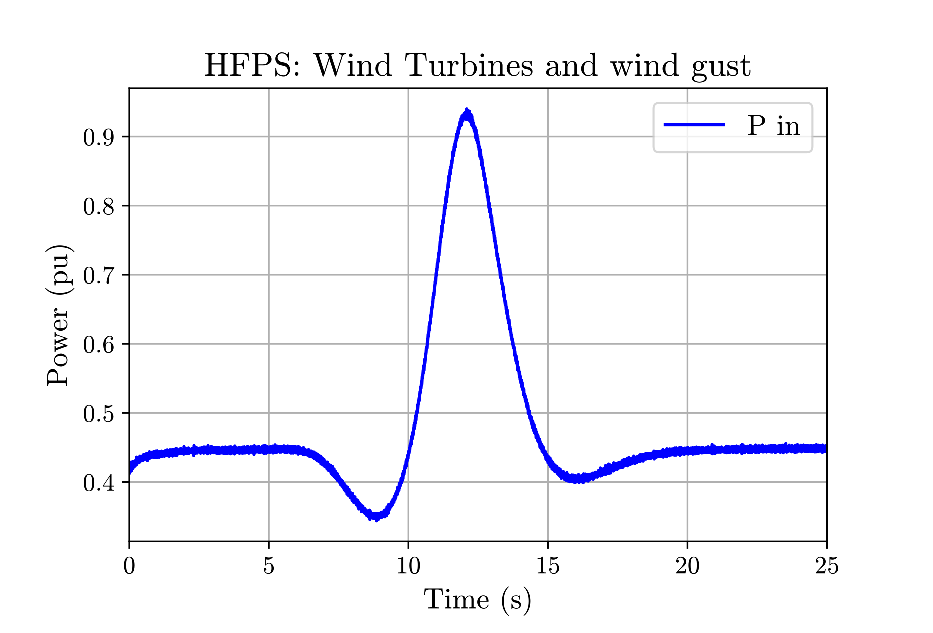
\includegraphics[scale=0.55]{figures/HFPS.eps}
        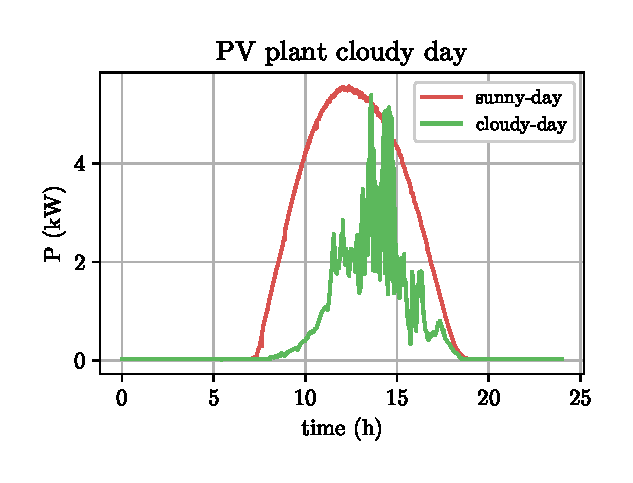
\includegraphics[scale=0.55]{figures/pv_cloudy-sunny.eps}
    \end{figure}
    
\end{frame}
%
%
\begin{frame}{¿Qué es el Power Smoothing?}
\begin{itemize}
    \item Acentuación de los problemas en redes débiles\\[1ex]
    \begin{itemize}
        \item Sistemas aislados, micro-redes \\[1ex]
        \item Grid Codes:
        \begin{itemize}
            \item PREPA (Puerto Rico): $10\% Pn/min$
            \item EirGrid (Irlanda): $30 MW/min$
            \item HECO (Hawai): $\pm2 MW/min$
            \item Denmark: $100 kW/s$ \\[1ex]
        \end{itemize}
        \item Tendencia a la penetración masiva de renovables \\[1ex]
        \item Tendencia a redes descentralizadas y autoconsumo \\[2ex]
    \end{itemize}{}
    \item Solución: Sistemas de almacenamiento energético (ESS)
    \begin{itemize}
        \item Super-condensadores  (SC)\\[1ex]
        \item Baterías (BESS)\\[1ex]
    \end{itemize}
    % Aquí habría que colocar aquí el esquema hardware
\end{itemize}
\end{frame}
%
%



\AtBeginSection[]
  {
     \begin{frame}<beamer>
     \frametitle{Contenidos}
     \tableofcontents[currentsection]
     \end{frame}
  }

\section[Líneas de investigación asociadas]{Líneas de investigación asociadas}
%%%%%%%%%%%%%%%%%%%%%%%%%%%%%%%%%%%%%%%%%%%%%%%%%%%%%%%%%%%%%%%%%%%%%%%%%%%%%%%%%%%%%%%%%
%
%
\subsection[]{El problema del dimensionado}
\subsection[]{El problema del control}
\subsection[]{El problema de la cuantificación}
%
%
%%%%%%%%%%%%%%%%%%%%%%%%%%%
%
%
\begin{frame}{Líneas de Investigación}
\begin{itemize}
    \item El problema del dimensionado
    \begin{itemize}
        \item Dimensionado del sistema de almacenamiento energético \\[1ex]
        \item Dimensionado de los convertidores \\[2ex]
    \end{itemize}
    \item El problema del control
    \begin{itemize}
        \item Algoritmos de control implementables en DSP \\[1ex]
        \item Ajuste de parámetros y ganancias del control \\[1ex]
        \item Control de potencia, control de SOC del EES \\[2ex]
    \end{itemize}{}
    \item El problema de la cuantificación
    \begin{itemize}
        \item Definición de índices y métricas \\[1ex]
        \item Retribución del servicio y estudio económico \\[1ex]
    \end{itemize}
\end{itemize}
\end{frame}
%
%
\section[Modelos Matemáticos]{Modelos Matemáticos}

%%%%%%%%%%%%%%%%%%%%%%%%%%%%%%%%%%%%%%%%%%%%%%%%%%%%%%%%%%%%%%%%%%%%%%%%%%%%%%%%%%%%%%%%%
%
%
%
%
%\subsection[]{Models Approaches}
\begin{frame}{Modelos Matemáticos}
Tratan de descomponer la potencia en términos que permitan distinguir entre potencia suavizada y no suavizada y los fenómenos que las producen. \\[2ex]
\begin{itemize}
    \item Métodos y técnicas off-line: Apropiados para el dimensioando \\[1ex]
    \begin{itemize}
        \item TSN-TSD: Trend Seasonality and Noise, Time Series Decomposition.\\[1ex]
        \item SSA: Singluar Spectrum Analysis\\[1ex]
        \item WD: Wavelet Denoisisng\\[2ex]
    \end{itemize}
    \item Métodos y técnicas on-line: Apropiados para el algoritmo de control\\[1ex]
    \begin{itemize}
        \item LPF: Low Pass Filtering \\[1ex]
        \item MA: Moving Average Filtering \\[1ex]
        \item RRF: Ramp-Rate Filtering \\[2ex]
    \end{itemize}{}
\end{itemize}
\end{frame}
%
%
%
%%%%%%%%%%%%%%%%%%%%%%%%%%%%%%%%%%%%%%%%%%%%%%%%%%%%%%%%%%%

\include{Preguntas}
\begin{frame}
  \titlepage
  \centering \bf{mfrancisco@us.es} %\\[2em]
  \quad
  \qrcode[height=1.5cm]{https://github.com/frcsmachado/1stphdws/blob/master/pdf_slides/Taller_Alumn_Doctorado.pdf}


\end{frame}

\end{document}
